We apply our algorithm to several different settings:
\begin{itemize}
\item Logistic regression where the MLE exists.  The gradient $\nabla \ell(\beta)$ can be calculated exactly in this setting and thus our algorithm is guaranteed to converge.  We compare the results to those attained by the \texttt{glm} function in R and compare the performance to stochastic approximation.  We choose a starting value for which Newton-Raphson fails.

\item Ising model where the MLE exists.  The gradient $\nabla \ell(\eta)$ must be approximated in this setting via MCMC.  Although our algorithm is not guaranteed to converge in theory, it is still effective in practice.  We again compare the performance to stochastic approximation.

\item Sampson's monastery data.  We revisit the exam from Section~\ref{S:MCMC-MLE} which
discussed how MCMC-MLE will struggle to converge when the starting value is far
from the true MLE.  The model used here is the simple Erd\H{o}s-R\'{e}nyi-Gilbert model 
described in Section~\ref{S:Erdos} with network statistic $g(y)$ equal to the total number of edges present.

\item ERGM with two-dimensional sufficient statistics on a 9-node undirected network.  
Here we explore cases where the MLE does and does not exist.  
Our algorithm finds the MLE when
exists, and finds the LCM MLE and its support when it does not.  These can then
be used to constructed one-sided confidence intervals for the natural parameters.
\end{itemize}

\section{Example: logistic regression}
We illustrate the application of our algorithm in the case of a logistic regression 
with a starting point far from the 
solution.  In such a case, the Hessian matrix is often near-singular and algorithms 
such as Newton-Raphson which rely 
on it will fail.  For classical SA with step size $1/k$, the magnitudes of the updates 
diminishes too quickly for 
the parameter estimates to approach the MLE in a reasonable amount of time.

The response vector $Y$ has components that are Bernoulli trials with mean vector $p$.  
The natural parameter is $
\theta_i = \log \left( \frac{p_i}{1-p_i} \right )$, which is modeled component-wise as 
a linear function of the 
predictors $1, x_1, \ldots, x_{q}$, so that
\begin{align*}
	\theta_i &= \beta_0 + \beta_1 x_{1i} + \beta_2 x_{2i} + \cdots + \beta_{q} x_{q
\,i} = \beta^T x_i \qquad
i = 1, \ldots, n
\end{align*}
where $\beta = (\beta_0, \ldots, \beta_{q} )^T$ and $x_i = ( 1, x_{1i}, \ldots, x_{q 
i})^T$.  

Defining the model matrix $M$ to be the $n \times (q+1)$ matrix with the $x_i$ as 
rows, we can express $\theta = M \beta
$.  This in turn allows us to reparameterize the exponential family  as one with $
\beta$ as the natural parameter 
vector and $M^T y$ the vector of statistics with log likelihood
\begin{align*}
		 \ell(\beta) &=  \beta^T (M^T y) - c(\beta),
\end{align*}
where $y$ is the vector of observed Bernoulli responses.
By \eqref{E:nabla ell}, the gradient is
\begin{align*}
	\nabla \ell( \beta ) &=  M^T y - \E_{\beta}(M^T Y) = M^T( y - \E_{\beta}(Y) ),
\end{align*}
where $\E_{\beta}(Y) = \frac{1}{1 + \exp(-M \beta)}$ can be calculated exactly.  This 
allows us to directly apply 
Theorem~\ref{Thm:Line Search works}.

Suppose we specify our true parameter value to be $\beta = (0, 2, 2, 1, 1, 0, 0, 0)^T$ 
and use 100 independent draws 
from a correlated multivariate normal distribution centered at 0 as our predictors to 
generate 100 independent 
Bernoulli trials.  
Fitting these data using the R function \texttt{glm}, we find the MLE of $\beta$ to be
\begin{align*}
	\betaMLE = (  0.635,  5.949, 1.273, 0.180, 1.006, 1.536, -2.252, -0.472 )^T,
\end{align*}
where the disparity to the true value of $\beta$ results from a relatively small 
sample size of $n=100$.
We use $\beta_0 = ( 5, 4, 3, 2, 1, 0, -1, -2)^T$ for the starting point for our line 
search algorithm, a point for 
which Newton-Raphson fails due to a nearly singular Hessian matrix.  

We measure the performance of our algorithm in terms of the total number of iterations 
used, where each iteration 
requires the evaluation of the gradient, $\nabla \ell( \beta_k + \alpha_k p_k )$.  
Typically, several iterations take 
place in an inner loop to find a step size $\alpha_k$ that meets the curvature 
condition \eqref{E:curvature mod}, a 
process that grows increasingly difficult as the estimates near the MLE since the 
rightmost term in \eqref{E:curvature 
mod} gets smaller in magnitude.  Once an acceptable step size is found, the parameter 
estimate $\beta_k$ is updated and 
a new search direction is determined, requiring another evaluation of the gradient.

Our algorithm took 54 iterations over 20 different search directions to get $\lVert 
\nabla \ell( \beta_k ) \rVert < 
0.01$ and arrive at an estimate for the MLE that differs from the \texttt{glm} result 
by 0.0117 in Euclidean distance 
(See Table~\ref{Table:Logistic}).  
Using the Polak-Ribi\`{e}re conjugate gradient method described in the previous 
section  resulted in comparably sharp 
MLE estimates (see Table~\ref{Table:Logistic}) in fewer iterations---28 over 11 search 
directions---a noticeable 
improvement. 

We also applied  SA with step size $1/k$ (setting $A=1$, $B=0$ in \eqref{E:SA step 
size}) from the same starting point 
$\beta_0$.  The choice of constants $A$ and $B$ in the step size is of course not 
likely to be optimal;
however, we want to apply SA without trial and error experimentation.  
After 10,000 iterations, the parameter estimates look nothing at all like the MLE (See 
Table~\ref{Table:Logistic}).  
The starting point $\beta_0$ is so far from the MLE and the step sizes so small that 
the algorithm does not converge in a reasonable amount of time.
Table~\ref{Table:step size} shows the first 20 step sizes used by SA and our line 
search. Our line search continues to 
use step sizes of relatively large magnitude even well into the process.  It should be 
noted that these 20 step sizes 
correspond to the first 20 iterations of SA but all 54 iterations of our line search 
algorithm since it spends several 
iterations finding an acceptable step size for each update.


% latex table generated in R 2.10.1 by xtable 1.5-6 package
% Tue May  4 17:37:01 2010
\begin{table}
\caption{Comparison of MLEs of $\beta$ for Example 1: MLE = \texttt{glm}, Steep = line 
search using steepest ascent, 
CG = line search using conjugate gradient, and SA =  SA with step size = $1/k$, 
terminated at 10,000 iterations,
$n$ = number of iterations.  Our 
proposed algorithm arrives at nearly identical MLE estimates to \texttt{glm}.}
\begin{center}
\begin{tabular}{rrrrrrrrrr}
  \hline
 & $n$ & $\beta[1]$ & $\beta[2]$ & $\beta[3]$ & $\beta[4]$ & $\beta[5]$ & $\beta[6]$ & 
$\beta[7]$ & $\beta[8]$ \\ 
True $\beta$ & & 0.000 & 2.000 & 2.000 & 1.000 & 1.000 & 0.000 & 0.000 & 0.000 \\ 
  $\hat{\beta}_{\textrm{MLE}}$ & & 0.635 & 5.949 & 1.273 & 0.180 & 1.006 & 1.536 & 
$-2.252$ & $-0.472$ \\ 
  $\hat{\beta}_{\textrm{Steep}}$ & 54 & 0.633 & 5.938 & 1.272 & 0.181 & 1.005 & 1.535 
& $-2.249$ & $-0.470$ \\ 
  $\hat{\beta}_{\textrm{CG}}$ & 28 & 0.631 & 5.936 & 1.272 & 0.181 & 1.003 & 1.532 & 
$-2.244$ & $-0.470$ \\    
  $\hat{\beta}_{\textrm{SA}}$ & $10^4$ & 1.280 & 10.619 & 5.588 & 4.005 & 2.478 & 
$-7.153$ & 1.255 & 0.264 \\ 
  \hline
\end{tabular}
\end{center}
\label{Table:Logistic}
\end{table}

\begin{table}
\caption{The first 20 step sizes used by  SA (with step size $1/k$) and our algorithm 
for Example 1.  The step sizes 
used by our algorithm do not diminish like $1/k$.
}
\begin{center}
\begin{tabular}{rrrrrrrrr}
  \hline
  $k$ & $\alpha_{\textrm{SA}} = 1/k$  & $\alpha_{\textrm{Steep}}$ & $\alpha_{\textrm
{CG}}$ \\ 
  \hline
1	&	1.000	&	0.192	&	0.192	\\
2	&	0.500	&	0.319	&	0.319	\\
3	&	0.333	&	0.403	&	0.416	\\
4	&	0.250	&	0.353	&	0.561	\\
5	&	0.200	&	0.380	&	0.491	\\
6	&	0.167	&	0.333	&	1.092	\\
7	&	0.143	&	0.420	&	0.359	\\
8	&	0.125	&	0.307	&	0.314	\\
9	&	0.111	&	0.442	&	0.275	\\
10	&	0.100	&	0.283	&	0.318	\\
11	&	0.091	&	0.483	&	0.278	\\
12	&	0.083	&	0.241	&	-	\\
13	&	0.077	&	0.745	&	-	\\
14	&	0.071	&	0.203	&	-	\\
15	&	0.067	&	1.224	&	-	\\
16	&	0.063	&	0.173	&	-	\\
17	&	0.059	&	2.510	&	-	\\
18	&	0.056	&	0.195	&	-	\\
19	&	0.053	&	0.944	&	-	\\
20	&	0.050	&	0.173	&	-	\\
  \hline
\end{tabular}
\end{center}
\label{Table:step size}
\end{table}



\section{Example: Ising model} \label{S:Examples:Ising}
In this example, we apply our gradient-based line search algorithm to an Ising model 
\citep{Ising} on a toroidal square 
lattice.  Ising models are exponential families where each entry in the square lattice 
takes the value of either zero 
or one.  A realized sample is shown in Figure~\ref{F:pottsimage}.  The sufficient 
statistic vector is two-dimensional, 
comprising the number of entries with value one and the number of ``neighbor'' entries 
with the same value.  Entries are 
considered ``neighbors'' if they are adjacent to one another horizontally or 
vertically (but not diagonally).  
\begin{figure}[h]
\begin{center}
\includegraphics[width=4.5in,keepaspectratio]{potts}
\end{center}
\caption{A realized sample from an Ising model on a $32 \times 32$ lattice with $\eta 
= \left(0, \log(1 + \sqrt{2}) 
\right)^T$.  This value of $\eta$ corresponds to the phase transition point, where 
the sample images are mostly one 
color with small but significant portions of the other color.  There is no preference 
for the dominant color to be 
white or black.}
\label{F:pottsimage}
\end{figure}

Here we describe the toroidal square lattice as an $n \times n$ matrix $Y$ and each 
entry as $Y_{ij}$, where $i$ and $j
$ take values in $1, \ldots, n$ considered as a cyclical set (addition is done modulo 
$n$).  The sufficient statistic, 
$g(y)$, has components:
\begin{align*}
	g_1(y) &= \sum_{i=1}^n \sum_{j=1}^n I(Y_{ij}=1), \\
	g_2(y) &= \frac{1}{2} \sum_{i=1}^n \sum_{j=1}^n 
				\bigl[ I(Y_{ij}=Y_{i-1,j}) + I(Y_{ij}=Y_{i,j-1}) \\
							&\qquad \qquad \qquad + I(Y_{ij}=Y_{i+1,j}) + I(Y_{ij}=Y_
{i,j+1}) \bigr ]
				,
\end{align*}  
where $I(\cdot)$ denotes the indicator function taking logical expressions to the 
numbers zero and one, false 
expressions to zero and true expressions to one.  

Because of the interdependence of neighboring entries in the lattice, there is no 
closed form expressing $\nabla \ell
( \eta)$ as in the logistic example.  Instead, we need to approximate $\nabla \ell
( \eta)$ using MCMC as described by 
\eqref{E:nabla ell approx}.  As discussed in Section~\ref{section:MCMC approx}, 
Theorem~\ref{Thm:Line Search works} 
cannot be applied directly, but as we demonstrate here, satisfactory estimates are 
still attained.  The MCMC draws are 
performed here using the Swendsen-Wang algorithm \citep{Swendsen-Wang:1987,Swendsen-
Wang:1990}, available in the contributed R 
package \texttt{potts} \citep{Geyer:potts}.

We choose $\eta = \left(0, \log(1 + \sqrt{2} ) \right)^T$ to generate a $32 \times 32$ 
lattice, which we will use as 
our observed data (Figure~\ref{F:pottsimage}).  This value for $\eta$ is of particular 
interest because it corresponds 
to the phase transition point \citep{Potts} and has been shown to be difficult to 
estimate \citep{Geyer:1990}.  In 
order to get a good estimate of the MLE to which we can compare our algorithm's 
results, we use 10 iterations of Newton-Raphson starting 
from the true value of $\eta$ so that we can be confident it will converge.

%%%% 1/25/11 - added Newton
%The Newton-Raphson update for optimization is
%\begin{align*}
%	\eta_{k+1} = \eta_k + \left [  \nabla^2 \ell (\eta_k) \right ]^{-1} \nabla 
%\ell (\eta_k).
%\end{align*}
%
%\hl{When $\eta_k$ is sufficiently close to the MLE, it has been shown to converge 
%quadratically (super-quadratically?)  Citation?.  
%Our benchmark MLE is computed using the Newton-Raphson for 10 iterations, starting at 
%the true value of $
%\eta$.  By iterating 10 times, we 
%know that the error of the attained estimated for the MLE will be \textbf{SMALL}.}

%%%%%%%%


We apply our line search algorithm to this data using an arbitrary initial value of $
\eta^{(0)} = ( 2, 0.001)$ and a 
fixed MCMC sample size of 10,000.  Our algorithm used 62 iterations (gradient 
evaluations) over 17 search directions to 
get  $\lVert \nabla \ell( \eta_k ) \rVert < 0.005$ and arrive at an estimate of the 
MLE that differs from Newton-Raphson
by 0.0037 (see Table~\ref{Table:Potts}).   Using the Polak-Ribi\`{e}re conjugate 
gradient method resulted in 
comparably sharp MLE estimates using 45 iterations over 7 search directions.  The 
total MCMC sample sizes used were $62\times10,0000 = 620,000$ and $45\times10,0000 = 
450,000$, respectively.

%> cat( "Total iterations:",i.total, "\n")
%Total iterations: 62 
%> cat( "Outer iterations:",i, "\n")
%Outer iterations: 18 
%> cat( "Inner iterations:",i.total - i, "\n")
%Inner iterations: 44 



\begin{table}
\caption{Comparison of MLEs for $\eta$ for Example 2: MLE = Newton-Raphson starting 
from the true $\eta$, Steep = 
line search using steepest ascent, CG = line search using conjugate gradient, and SA = 
SA with step size = $1/k$.  All 
algorithms converged.}
\begin{center}
\begin{tabular}{rrrrrrlrr}
  \hline
%    &  &  &  & \multicolumn{1}{c}{inner}\\
  \multicolumn{1}{c}{} & 
  \multicolumn{1}{c}{MC Samples} &
  \multicolumn{1}{c}{$\eta[1]$} &
  \multicolumn{1}{c}{$\eta[2]$} \\
%  & \multicolumn{1}{c}{loop }\\
    &  \multicolumn{1}{c}{(thousands)} &  &  & \\
  \hline
True $\eta$  & & 0.000 & 0.881 \\ 
  $\hat{\eta}_{\textrm{MLE}}$ & & $-0.007$ & 0.896 \\ 
  $\hat{\eta}_{\textrm{Steep}}$ & 620 & $-0.011$ & 0.895 \\ 
  $\hat{\eta}_{\textrm{CG}}$ & 450 & $-0.008$ & 0.895 \\ 
  $\hat{\eta}_{\textrm{SA}}$ & 1368 & $-0.010$ & 0.895 \\ 
   \hline
\end{tabular}
\end{center}
\label{Table:Potts}
\end{table}

We also applied SA, again with step size $1/k$ from the same starting point $\eta^
{(0)}$, and used
a MCMC sample size of 1,000 for gradient calculation.  
Here SA converged in 1368 iterations or 1,368,000 MC samples, comparable to our 
algorithm (see Table~\ref{Table:Potts}).  Table~\ref{Table:Potts step 
size} shows the first 17 step sizes used by SA and our line search.  The step sizes 
used by our line search are 
initially very small compared to $1/k$, but stay in a range of about $1/300$ to 
$1/3000$.  So, the $1/k$ step size used 
by SA in fact occasionally satisfies our curvature condition when $k$ is large. 

\begin{table}
\caption{The first 17 step sizes used by SA (with step size $1/k$) and our algorithm 
for Example 2.  The step sizes 
used by our algorithm are initially much smaller than $1/k$.}
\begin{center}
\begin{tabular}{rrrrrrrrr}
  \hline
  $k$ & $\alpha_{\textrm{SA}} =1/k$  & $\alpha_{\textrm{Steep}}$ & $\alpha_{\textrm
{CG}}$ \\ 
  \hline
1	&	1.0000	&	0.0029	&	0.0029	\\
2	&	0.5000	&	0.0005	&	0.0005	\\
3	&	0.3333	&	0.0017	&	0.0017	\\
4	&	0.2500	&	0.0013	&	0.0045	\\
5	&	0.2000	&	0.0017	&	0.0007	\\
6	&	0.1667	&	0.0011	&	0.0002	\\
7	&	0.1429	&	0.0021	&	0.0015	\\
8	&	0.1250	&	0.0009	&		\\
9	&	0.1111	&	0.0020	&		\\
10	&	0.1000	&	0.0007	&		\\
11	&	0.0909	&	0.0018	&		\\
12	&	0.0833	&	0.0006	&		\\
13	&	0.0769	&	0.0013	&		\\
14	&	0.0714	&	0.0006	&		\\
15	&	0.0667	&	0.0007	&		\\
16	&	0.0625	&	0.0003	&		\\
17	&	0.0588	&	0.0013	&		\\
  \hline
\end{tabular}
\end{center}
\label{Table:Potts step size}
\end{table}

%\subsection{Side note: MLE distribution for Ising models}
An interesting side note about the MLE distribution for Ising models
and their generalization to 
more than two colors called Potts models is that for these moderate size lattices (including
$32 \times 32$ or even $100 \times 100$), the distribution appears to be skewed and 
biased \citep{Composite}.  In the sample run above, the MLE happens to be very close 
to the true parameter value.  However, by calculating MLEs for 1000 different $32 \times 32$
observed lattices, we find the empirical average for the $\eta[2]$ component to be $0.856$ with a
standard error of 0.036.  The histogram for $\eta[2]$ component of the MLE 
based off of 1,000 simulations is shown in Figure~\ref{F:ising-hist}. 

\begin{figure}[h]
\begin{center}
\includegraphics[width=4.5in,keepaspectratio]{ising-hist}
\end{center}
\caption{Histogram of the $\eta[2]$ component for 1000 MLEs for 
an Ising model on a $32 \times 32$ lattice with $\eta = \left(0, \log(1 + \sqrt{2}) 
\right)^T$.  The vertical line is at $\log(1 + \sqrt{2}) = 0.881$. }
\label{F:ising-hist}
\end{figure}

%If we want to use 100 different observed data sets to estimate our MLE 
%distribution (that is, we will approximate MLEs for each of the 100 data sets), and 
%we will first need to generate 100 different observed samples.  Then, for each sample 
%we will want to MCMC sampling to maximize the log-likelihood ratio, $r( \theta, 
%\theta_0)$.  The beauty here is that in fact we can generate MCMC samples only once 
%(for a reasonable large size, say 100,000) and then use these to approximate the log-
%likelihood ratio.
%
%
%\begin{align*}
%%\theta_{MLE} = (0.004626115, 0.003245121, -0.001108131, 1.06203 )^T
%%\theta_{MLE} = (0.00463, 0.00325, -0.00111, 1.062 )^T
%\end{align*}
%with a standard deviation of 0.028 for $\theta_*$ (the sample standard deviation of 
%the 455 $\theta$ values we calculated).
%
%So, the mean of the MLEs we calculate is significantly lower than the true value of 
%1.098.

\section{Example: Sampson's monastery data}
As discussed in Section~\ref{S:MCMC-MLE}, the MCMC-MLE may struggle to converge when the 
starting value is far from the true MLE.  This was illustrated on Sampson's monastery data set with the Erd\H{o}s-R\'{e}nyi-Gilbert model with network statistic $g(y)$ equal to 
the total number of edges present.
The observed network, depicted in Figure \ref{F:Sampson}, is directed with 18 actors and 
88 ties present out of $18 \cdot 17=306$ possible ties.  The true MLE is equal to 
\begin{align*}
	\etaMLE = \logit\left( \frac{g(\yobs)}{n(n-1)}\right) = \logit \left( \frac{88}{306}\right ) = -0.9072.
\end{align*}
With $\eta^0 = 1$, the MCMC-MLE approximated log likelihood ratio (using 100,000 samples) 
cannot be maximized, as shown in Figure~\ref{F:MCMC-MLE}.
We start from this same initial value, using the \texttt{simulate.formula} function
from the \texttt{ergm} package in R to generate 200 MCMC samples, $g(Y_1), \ldots, g(Y_
{200})$, with each sample spaced 1000 apart from one another.

It took our algorithm 24 iterations over 4 different search directions to get $\lVert 
\nabla \ell( \eta_k ) \rVert < 0.05$ and arrive at an estimate for the MLE of  $-0.9145$.  The intermediate steps are presented in Table~\ref{T:Sampson redo}.  That the final estimate of $-0.9145$ is not closer to the true MLE of $-0.9072$ than the previous estimate of $-0.9042$ is due to MC error.  The runtime was 4 minutes on a 2GHz computer.

\begin{table} \label{T:Sampson redo}
\caption{
Long range algorithm applied to Sampson's 
mastery data.  The starting point of $\eta^0 = 1$ can be thought of as ``far" from the
true MLE of $-0.9072$.  The inner loop count is the number of iterations spent searching for an $\alpha_k$ that meets the curvature condition.  
}
\begin{center}
\begin{tabular}{rrrrrrlrr}
  \hline
    &  &  &  & \multicolumn{1}{c}{inner}\\
  \multicolumn{1}{c}{$k$} & 
  \multicolumn{1}{c}{$\eta_k$} &
  \multicolumn{1}{c}{$\lVert \nabla \ell(\eta_k) \rVert$} &
  \multicolumn{1}{c}{$\alpha_k$} &
  \multicolumn{1}{c}{loop }\\
    &  &  &  & \multicolumn{1}{c}{count}\\
  \hline
   0 &  $1.0000$ & 136.940 &  0.012 & 9 \\
   1 & $-0.6595$ & 16.600  &  0.014 & 3 \\
   2 & $-0.8846$ & 2.265   &  0.009 & 11 \\
   3 & $-0.9045$ & 1.140   &  0.009 & 1 \\
   4 & $-0.9145$ & 0.010   &  & \\
   \hline
\end{tabular} \label{T:Sampson redo}
\end{center}
\end{table}


\section{Example: 9-node network}
We now dive into the more difficult cases for ERGMs where the MLE may not exist.
Like \citet{Handcock:degeneracy, Rinaldo:2009}, we focus on small networks (9 nodes or 
fewer) with only two or three network statistics.  
Because we need to compare our algorithm to the truth---whether or not the MLE exists, 
and what its value
is if it does---we work with networks for which it is feasible to evaluate the likelihood
function.  For an undirected 9-node network this requires a summation over  $2^{{9\choose 2}}$, or about 69 billion different graphs.  Determining the existence of the MLE
requires knowledge of the convex support of the sufficient statistics.  See Appendix~\ref{A:Triangle count} for our approach to enumerate all possible graphs in a 9-node network with counts of three network statistics: edges, two-stars, and triangles.

%We also use a model with 
%a three-dimensional statistic comprising edges, triangles, and two-stars to get a 
%greater variety of empirical faces and normal cones.

For comparison purposes with \citet{Rinaldo:2009}, we focus first on a model with the number 
of edges and triangles as the natural statistics.  A two-dimensional statistic 
naturally also lends itself to more easily interpretable figures.  The relevant convex support for this model is displayed in Figure~\ref{F:g9-hull}.  Although there are nearly 69 billion
possible graphs, there are only 444 possible combinations of edges and triangles.
Let the space of these sufficient statistics be denoted $\TT = g(\YY)$.
The summation in the normalizing constant \eqref{E:kappa} over all graphs in $\YY$ can in fact be simplified
 to a weighted sum over the 444 points in $\TT$ as follows:
\begin{align*}
	\kappa(\eta) = \sum_{y \in \YY} e^{\inner{g(y),\eta} } = 	\sum_{t \in \TT} e^{\inner{t,\eta} } \nu(t)
\end{align*}
where $\nu(t)$ is the frequency of the network statistic $t$ across all $y \in \YY$.  
This does require knowing $\nu(t)$ for all $t \in \TT$, something we calculate
and save to file in our enumeration of all possible graphs.

In fact, we will find it easier to work directly with the distribution of the sufficient
statistic $T=g(Y)$:
\begin{align*}
	P_\eta(T=t) 	&= \sum_{y \in \YY: g(y) = t} P_\eta(Y= y ) \\
		 		&= \sum_{y \in \YY: g(y) = t} \frac{1}{\kappa(\eta)} e^{\inner{g(y),\eta} } \\
				&= \sum_{y \in \YY: g(y) = t} \frac{1}{\kappa(\eta)} e^{\inner{t,\eta} } \\
				&= \frac{1}{\kappa(\eta)} e^{\inner{t,\eta} } \nu(t).
%	P_\eta(T=t) = \frac{1}{\kappa(\eta)} e^{\inner{\eta, t}} \quad t \in \TT
\end{align*}
%The log likelihood $\ell(\eta)$ can then be expressed
%\begin{align*}
%	\ell( \eta) &= \inner{g(\yobs), \eta} - \log \kappa( \eta ) \\
%				&=  \inner{g(\yobs), \eta} - \log \sum_{y \in \YY}e^{\inner{t(y),
%\theta}}.
%\end{align*}

We can then calculate exact values for the gradient of the log likelihood $\nabla \ell(\eta)$ by \eqref{E:nabla ell},
\begin{align*}
	\nabla \ell (\eta) &= g(\yobs) - \E_\eta g(Y)\\ 
					  &= g(\yobs) - \E_\eta T \\
					  &= g(\yobs) - \sum_{t \in \TT} t P_\eta(T = t) \\
					  &= g(\yobs) - \frac{1}{\kappa(\eta)}  \sum_{t \in \TT} t e^{\inner{t,\eta} } \nu(t).
\end{align*}

To address concerns for overflow possibilities where $e^x$ can become too large, we 
can subtract $a = \max_t \inner{t, \eta}$ from each term in the summations, so that
\begin{align*}
	\nabla \ell (\eta) &= g(\yobs) - \frac{1}{\sum_{t \in \TT} e^{\inner{t,\eta}-a} \nu(t)}  \sum_{t \in \TT} t e^{\inner{t,\eta}-a} \nu(t).
\end{align*}
The second derivative of the log likelihood $\nabla ^2 \ell(\eta)$ can also be 
expressed in term of the sufficient statistic.  By \eqref{E:nabla2 ell},
\begin{align*}
	\nabla ^2 \ell(\eta) &= - I(\eta) = -\Var_\eta g(Y) \\
	&= -\Var_\eta T \\ 
	&= - \E (T - \E_\eta T)( T - \E_\eta T)^T \\
				&= - \sum_{t \in \TT} (t - \E_\eta T)(t - \E_\eta T)^T P(T=t)\\
				&= - \frac{1}{\kappa(\eta)} \sum_{t\in \TT}
					(t - \E_\eta T)(t - \E_\eta T)^T e^{\inner{t,\theta}} \nu(t).
\end{align*}
The same adjustment for overflow as used for $\nabla \ell(\eta)$ can be applied here.

Being able to evaluate $\nabla \ell(\eta)$ and 
$\nabla^2 \ell(\eta)$ exactly is useful when searching directly from MLEs;
optimization routines such as \texttt{trust} \citep{trust:R} in R will use these
as inputs.  

For the 9-node undirected network model with edge and triangle sufficient statistics,
we are now equipped with the knowledge of the convex support and a log likelihood we 
can evaluate and numerically maximize.  The linear programming functions in 
\texttt{rcdd} will determine whether an observed network falls on the boundary 
or interior of the convex support.  These will allow us to establish the ``truth" 
against which we can compare our algorithm.

The key difference between our work here and the approaches of 
\citep{Handcock:degeneracy,Rinaldo:2009} is that our algorithm does not assume
knowledge of the convex support $C$ and thus must determine ``on the fly" whether
or not the MLE exists.  
We do take liberty with two short cuts in the application of our algorithm to make 
our analysis cleaner:
\begin{enumerate}
\item MC sampler.  We use a perfect Monte Carlo sampler to generate our draws \\
$g(Y_1), \ldots, g(Y_m)$ from the distribution with parameter $\eta$, rather than a 
MCMC sampler. \\
 Although we have replicated the results of the algorithm using the 
 \texttt{simulate.formula} MCMC sampler provided in the R package \texttt{ergm} 
 \citep{ergm:R}, we wish to identify here what 
issues would still be present even with a perfect MC sampler, which we can easily build for 
this small network since the likelihood function can be evaluated.  Some issues 
related to the challenges of MCMC sampling for ERGMs are discussed in 
\citep{ergm,Morris:2008}; we do not concern ourselves with these issue here.

\item Step length search.  The search for the step length $\alpha_k$ that satisfied the 
curvature condition \eqref{E:Wolfe-ll} can be time consuming, as discussed in
Section~\ref{S:MCMC approx} and evident in our previous examples.
Here we use our ability to evaluate the gradient function $\nabla \ell(\cdot)$ exactly;  
we solve for the value that sets $\nabla \ell( \eta_k + \alpha_k p_k)^T p_k = 0$ 
using a simple root-finding algorithm.  That is, for a given 
direction $p_k$, we find the step size that maximizes the log likelihood in that 
direction.

We do not use this shortcut in any other portions of our approach that 
require $\nabla \ell(\cdot)$, 
such as updating search directions $p_k$.

\end{enumerate}
We believe that neither of these undermine the validity of our overall methodology, 
though they undoubtedly simplify and speed up its application.

%We now return to the examples from Section~\ref{S:Example}.  We describe the relevant 
%R functions, which unless otherwise noted are in the \texttt{rcdd} package \citep{rcdd:R}.



%%%%%%%%%%%%%%%%%%%%%%%%%%%%%%%%%%%%%%%%%%%%%%%%%%%%%

%%%%%%%%%%%%%%%%%%%%%%%%%%%%%%%%%%%%%%%%%%%%%%%%%%%%%%%%
\subsection{Two-dimensional sufficient statistic}\label{S:example 2dim}
The MLE for an exponential family model will exist if and only if the observed 
statistic lies in the interior of the polyhedral convex support $C$, which is the sail-shaped polytope in Figure \ref{F:g9-hull}. Here, $C$ has six sides (and six vertices).

\subsection{Case: MLE exists}
Suppose the observed network data has 29 edges and 47 triangles.  Then $g(\yobs) = (29,47)$
lies in the interior of the convex support as depicted in Figure \ref{F:MC cloud} 
(top) and the MLE exists.
Our algorithm, arbitrarily starting at the natural parameter value of $\eta = (0,0)$, 
generates Monte Carlo samples from the model with this initial parameter value.  As 
the algorithm climbs the log likelihood surface, 
the cloud of sample points will move towards 
the observed statistic and eventually engulf it.  
When the value for $\eta$ is equal to the MLE, the mean of the MC sample points will 
equal $(29,47)$(see Figure \ref{F:MC cloud} (bottom)).  
\begin{figure}[!ht]
\centering
%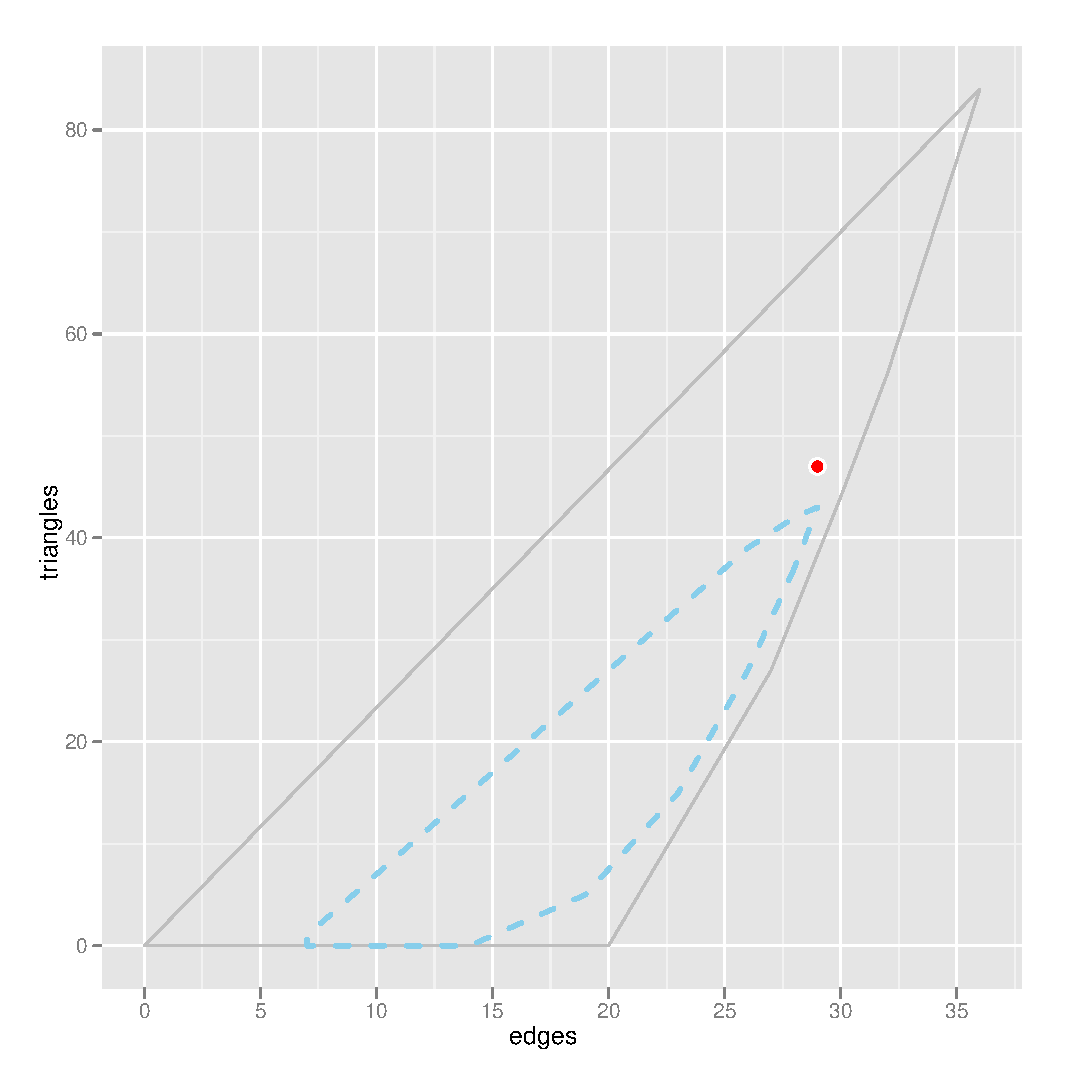
\includegraphics[height=2.8in,width=2.8in]{Figures/MCsample-far}
%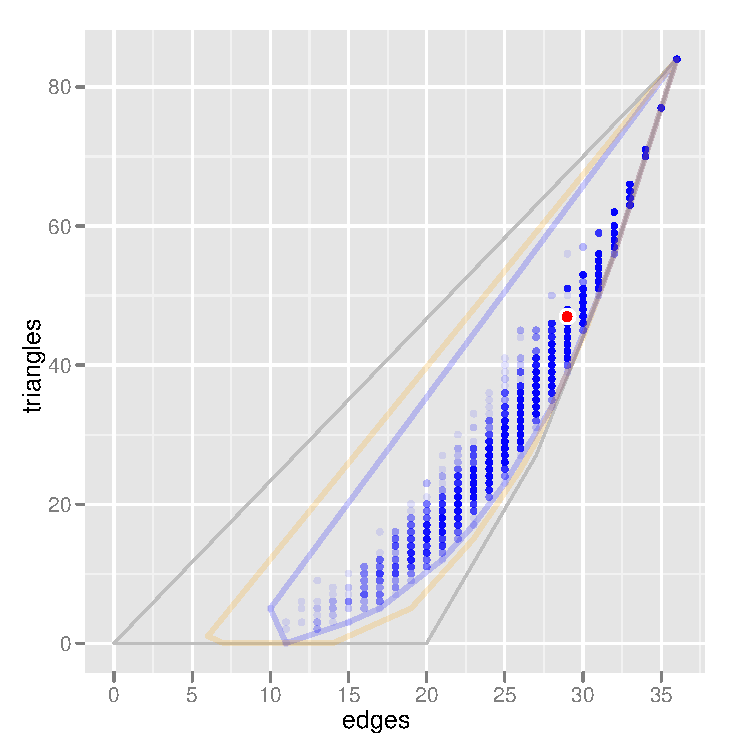
\includegraphics[height=2.8in,width=2.8in]{Figures/MCsample-MLE}
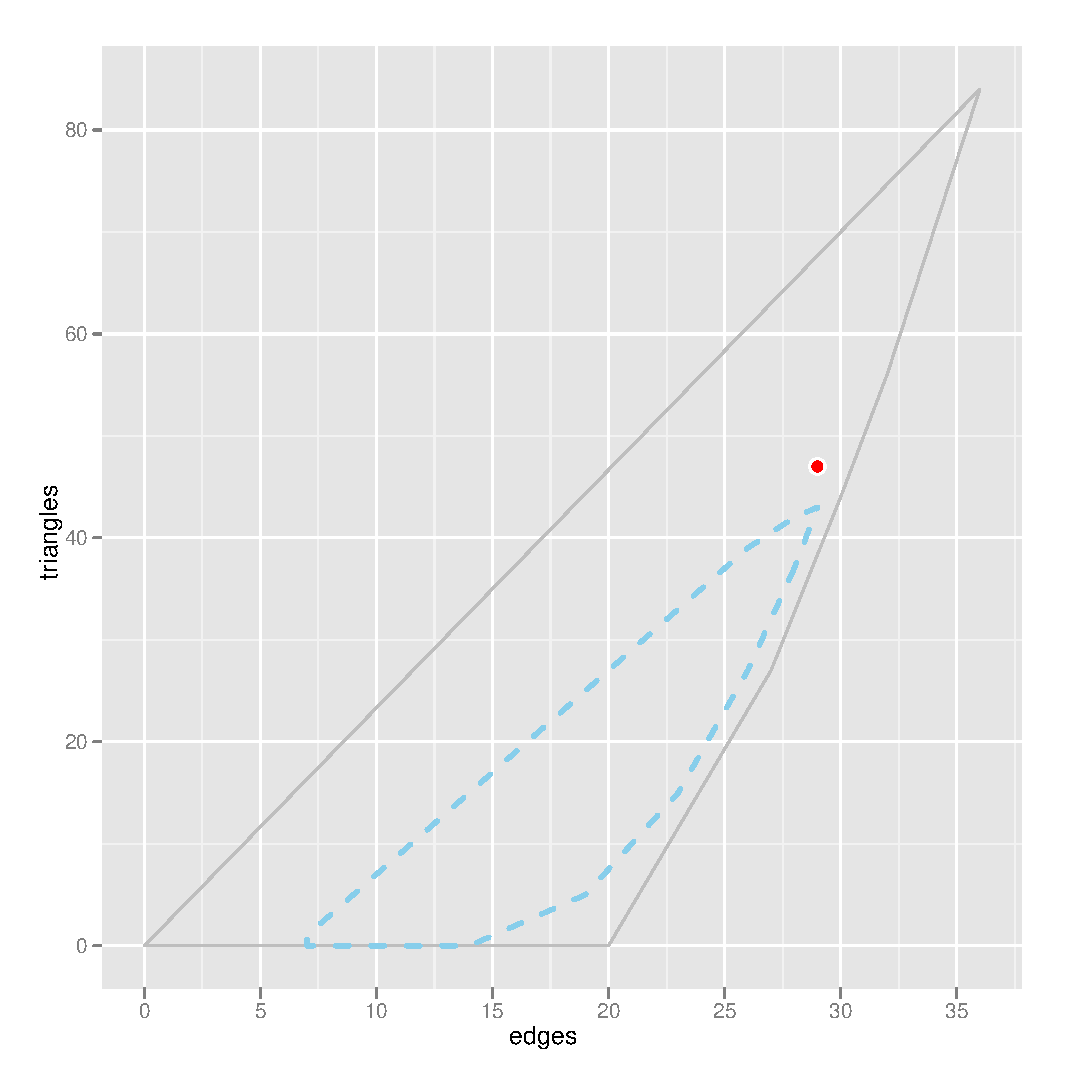
\includegraphics[width=3.8in]{Figures/MCsample-far}
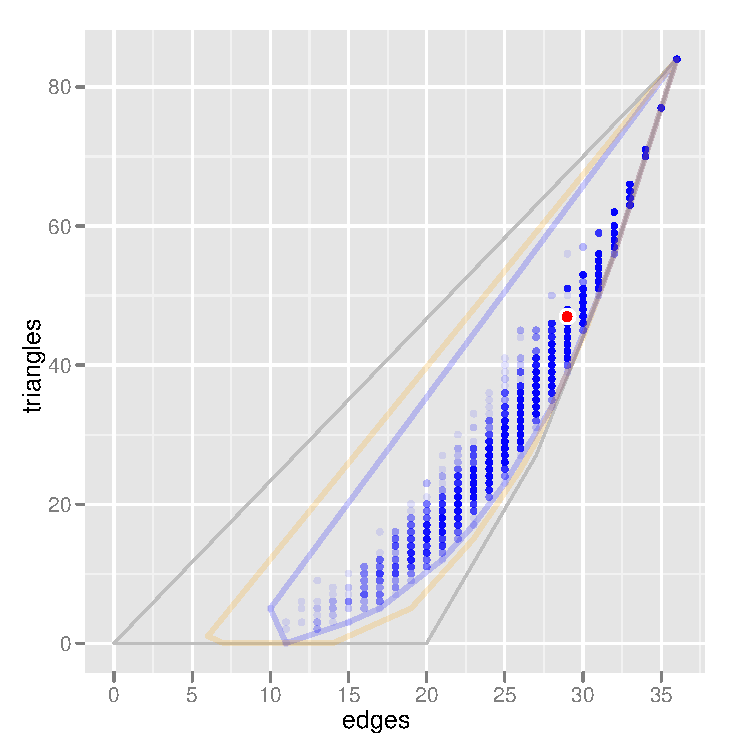
\includegraphics[width=3.8in]{Figures/MCsample-MLE}
\caption{The network statistics for 10,000 Monte Carlo samples generated from models 
with the natural parameter $\eta$ set to $(0,0)$ (top) and the MLE $(-0.389, 0.418)$ 
(bottom).  The observed data has network statistics of $(29,47)$, depicted by the 
larger point with white outline.  When $\eta$ is the MLE, the observed statistic is 
exactly the mean of the MC sample points generated from the model with this parameter 
value. }
\label{F:MC cloud}
% (-0.3890151, 0.4177752) % from trust
\end{figure}
For this problem, the MLE for $\eta$ is found to be
\begin{align*}
\etaMLE = (-0.389, 0.418),
\end{align*}
which matches the results we get from applying \texttt{trust} to numerically
maximize the log likelihood function.

\subsection{Case: MLE does not exist; observed statistic on one-dimensional face}
Suppose the observed network has network has 31 edges and 50 triangles.  Then 
$g(\yobs) = (31,50)$ lies on the boundary of the convex support as depicted in 
Figure \ref{F:MC face}.  To be precise, the observed network statistic $(31,50)$ lies 
on the interior of a line segment on the boundary of the convex support with 
end points $(30,44)$ and $(32,56)$. 
By Theorem~\ref{Thm:MLE rint}, it is clear that the MLE does not exist.

Our algorithm begins as before, generating MC sample point clouds to explore the 
space, as depicted in Figure \ref{F:MC face} (top).  Because the convex 
support is not assumed to be known, 
the algorithm cannot determine at the outset that the MLE does 
not exist; rather, it can only generate more sample point clouds as it climbs the log 
likelihood surface, with successive point clouds moving towards the observed statistic.
Eventually, the observed statistic will lie exactly on the boundary of a point cloud.
When this occurs, the algorithm must 
\begin{enumerate}
\item determine empirically the face $F$ on which the observed statistic lies in the 
relative interior of,
\item decide if $F$ is in fact the boundary of the convex support $C$.
\end{enumerate}  

The first task can be done using the linear programming functions provided to us in 
the \texttt{rcdd} package and described in Chapter~\ref{Chapter:Linear programming}.  The second task turns out to be very difficult to do.  
For now, we assume that if a substantial portion of the sample points generated, say 
60\%, land on this empirically determined face $F$, then it is in fact a boundary of 
the convex support $C$.  


In this example, the algorithm uses the \texttt{linearity} function to determine empirically that three points from the MC sample---$(30,44)$, $(31,50)$, 
and $(32,56)$---lie on a one-dimensional face, as depicted in Figure \ref{F:MC face} 
(bottom).  If less than 60\% of the sample points land on this empirical face, the 
algorithm continues to sample, trying to get a sample point cloud even closer to the 
observed statistic.  We choose such a high proportion for a cut off to eliminate---or 
at least, greatly reduce---the possibility of misidentifying a boundary.
(We deal later with a case where 100\% of the MC sample points form a face which is 
\emph{not} on the boundary of $C$.)
\begin{figure}[!ht]
\centering
%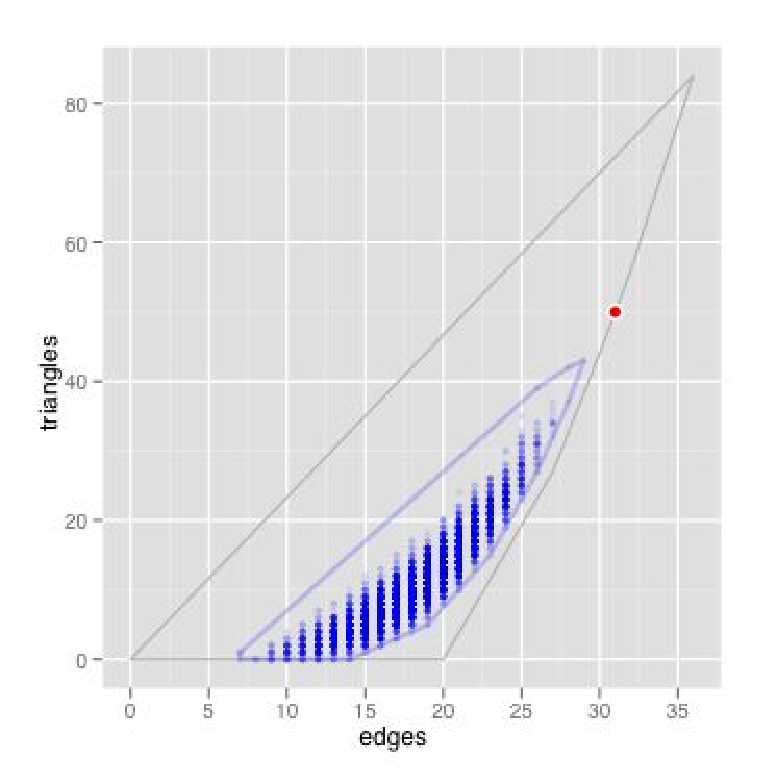
\includegraphics[height=2.7in,width=2.7in]{Figures/MCsample-boundary}
%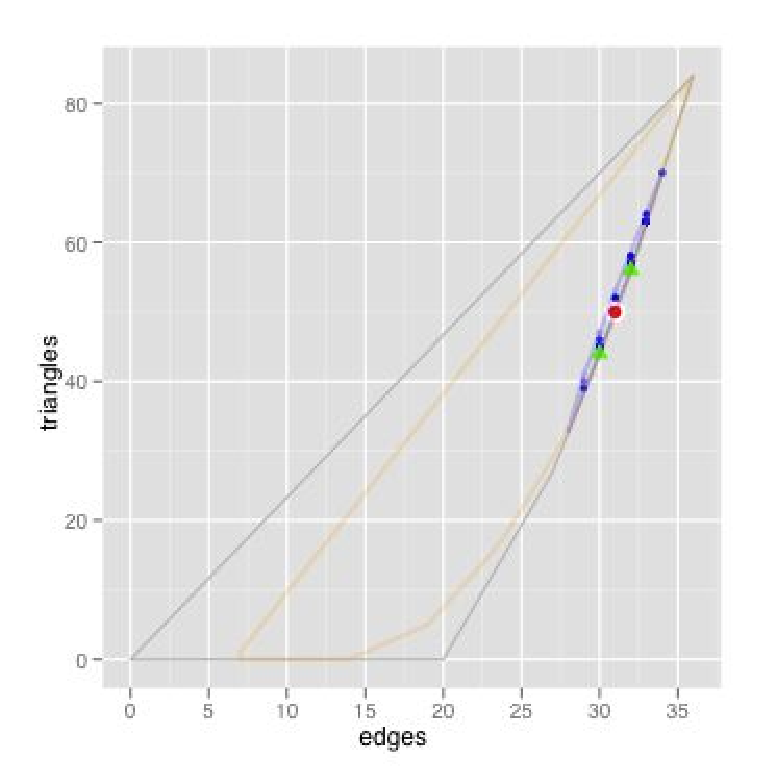
\includegraphics[height=2.7in,width=2.7in]{Figures/MCsample-77face}
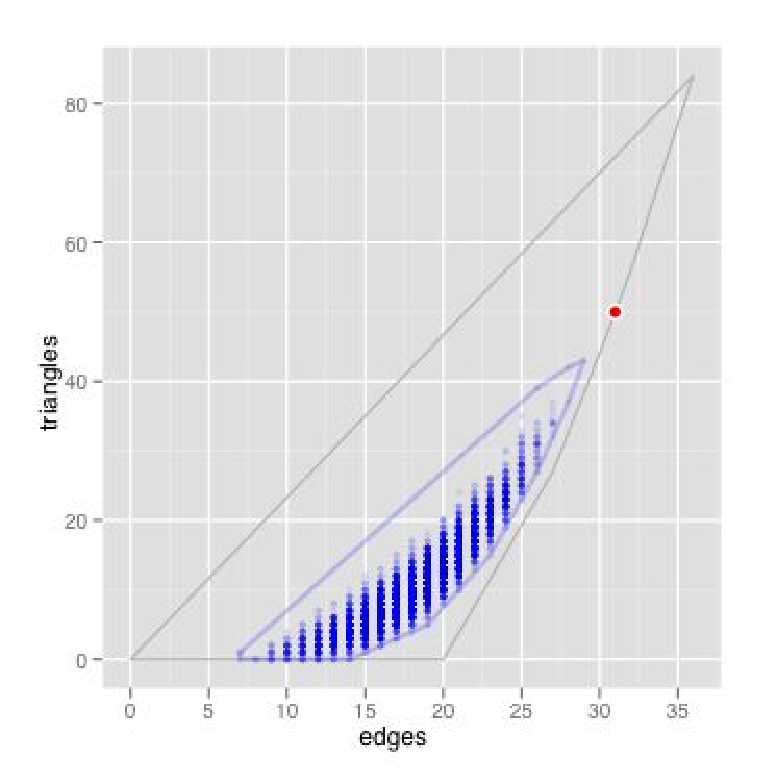
\includegraphics[width=3.7in]{Figures/MCsample-boundary}
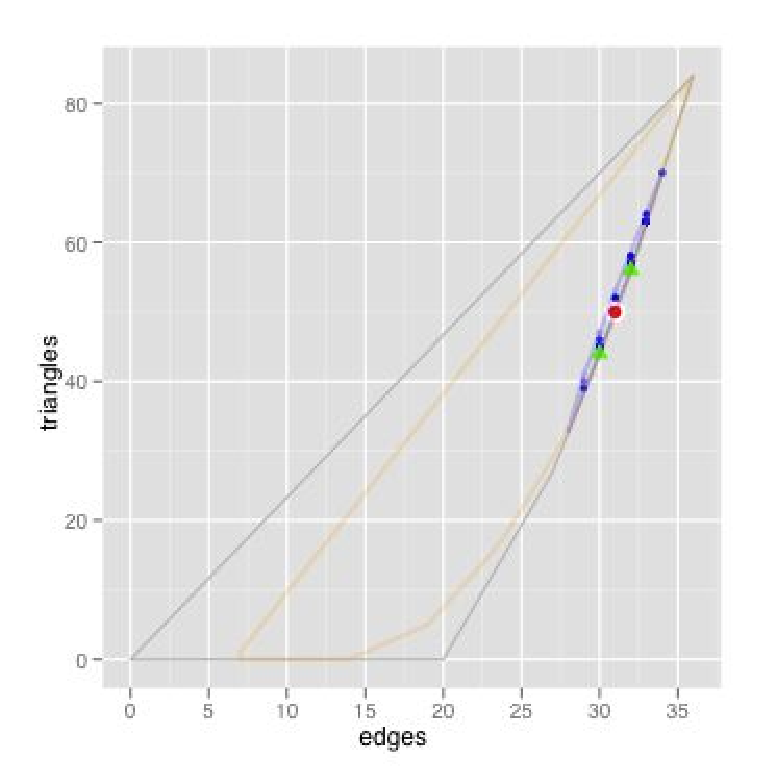
\includegraphics[width=3.7in]{Figures/MCsample-77face}
\caption{The network statistics for 10,000 Monte Carlo samples for the model with 
observed network statistic $(31,50)$, depicted by the larger point with white 
outline, lying on the boundary of the convex support (top).
In the bottom figure, the algorithm has identified a face defined by $(30,44)$, 
$(31,50)$, and $(32,56)$, marked by triangles in the figure (the triangle for 
$(31,50)$ is not visible since it is the observed statistic).  
Here, 77\% of the MC sample points fall on these three points.  The 
lighter colored polytope is the convex hull of all previously sampled points.
}
\label{F:MC face}
\end{figure}

By identifying the empirical face $F$ on whose relative interior the observed 
statistic lies, 
the algorithm has not only concluded that the MLE does not exist in the conventional 
sense, it has also defined $F$ as the convex support for the new limiting conditional 
model for which the MLE must exist by Theorem~\ref{Cor:spanL} and \ref{Thm:C-H}.
The algorithm then maximizes this new exponential family using the same 
iterative approach as before.  The gradient of the LCM log likelihood is approximated 
using \eqref{E:nabla ell approx LCM},
\begin{align*}
	\nabla \ell( \eta )^{LCM} \approx g(\yobs) - \frac{1}{k} \sum_{i=1}^k g(Y_{(k)})
\end{align*}
where $g(Y_{(1)}), \ldots, g(Y_{(k)})$ is the subsample of the MC sample points 
restricted to the empirical face, $(30,44)$, $(31,50)$, and $(32,56)$ in this case.  
The maximizer of this log likelihood $\etaLCM$ is found by the algorithm to
be
\begin{align*}
\etaLCM = (120.9, -20.1).
%(120.91090 -20.12784)
\end{align*}
\hl{The LCM, however, is not identifiable, since the support is now only one-dimensional 
compared to two in the original model. } 
That is, there must exist a constancy space of this new model, $\Gammalim$, such that 
\begin{align} \label{E:Gammalim}
\ell( \eta + \gamma )^{LCM} = \ell( \eta )^{LCM}
\end{align}
for any $\gamma \in \Gammalim$.

The empirical face $F$ and the observed statistic also define a normal cone by Theorem~\ref{Thm:DOR}, which in this case is a single direction, 
\begin{align*}
	\delta = (6,-1)
\end{align*}
and is also a GDOR by definition, since it is the only direction in the 
relative interior of the normal cone which is not a vector subspace.  The normal 
cone is derived by the methods described in Chapter~\ref{Chapter:Linear programming}.
By Corollary~\ref{Cor:strictly increasing}, a GDOR $\delta$ is a direction along which the log likelihood function is strictly increasing, and by 
Theorem~\ref{Thm:LCM}, we know that
\begin{align} \label{E:GDOR lim}
	\lim_{s \to +\infty} \ell( \etaLCM + s \delta) = \sup_{\eta} \ell(\eta).
\end{align}


The GDOR $\delta$ of the original model is also a direction of constancy for the new 
model [WHY].  
%Then by \eqref{E:Gammalim} and \eqref{E:GDOR lim}, note that $\ell(\etaLCM + \gamma + 
%s \delta)$ goes off to $+\infty$ as $s$ increases.  

In order to construct a one-sided confidence intervals, we need to find the value of 
$s$ for which the the distribution indexed by $\etaLCM + s \delta$ assigns a probability
of 0.05 to the event that a sample falls on the face of interest is.  That is,
\begin{align*}
P_{\etaLCM + \gamma + s \delta}(g(Y) \in F ) = 0.05.
\end{align*}
Although we cannot evaluate the probability function above, we can generate MC samples 
of $g(Y_1), \ldots, g(Y_m)$ from the distribution with parameter $\etaLCM + s 
\delta$ and see for what value of $s$, 5\% of the sample lies in the 
empirical face we found.  
\hl{CHARLIE SAYS: USE IMPORTANCE SAMPLING FORMULA---MORE EFFICIENT}

Some numerical calculations shows that the original exponential family index by
 $\eta = (9.14, -1.50)$ puts 5\% of the MC sample on this face.  
Expressing this as a non-simultaneous 95\% confidence intervals for the components of $\eta$,
\begin{align*}
	[9.14, +\infty)\\
	(-\infty, -1.50],
\end{align*}
where the direction of the interval for the second component is flipped because the 
second component of $\delta$ is negative.

We also applied a trust optimization routine on the original log 
likelihood in attempt to maximize it.  The maximum of course does not exist, but
because the surface flattens so much, the routine returns a value it perceives as a maximizer,  
\begin{align*}
 	\hat{\eta}_{\textrm{trust}} = (135.6, -22.6),
 \end{align*}
which are well within our confidence intervals.


%Alternatively, in mean value parameterization, the
%non-simultaneous 95\% confidence intervals for the edge and triangle parameters are
%\begin{align*}
%	[29.7, 31]\\
%	[44.1, 50],
%\end{align*}
%where the upper bounds are the observed data and hence the MLE in this parameterization.
%%Incidentally, the mean parameterization of $\hat{\eta}_{\textrm{trust}}$ is $(31,50)$, 
To summarize, our algorithm has realized the MLE for this model does not exist.
It has found the one-dimensional face $F$ with end points $(30,44)$  
and $(32,56)$ on which the observed statistic lies, where $F$ is also the
convex support of the LCM.  The algorithm has also identified a GDOR $\delta = (6,-1)$
along which the log likelihood is strictly increasing.  Finally, the algorithm 
has returned the end points for one-sided confidence intervals for the natural
parameters.


%%%%%%%%%%%%%%%%%%%%%%%%%%%%%%%%%%%%%%%%%%%%%%%%%%%%%
\subsection{Case: MLE does not exist; observed statistic on zero-dimensional face}
If the observed network has statistic $g(\yobs) = (27, 27)$,  then 
$g(\yobs)$ is an \emph{extreme point} 
of the convex support $C$ (it is one of the six defining vertices of $C$, depicted by
a square point in Figure~\ref{F:g9-hull}).  In this case, the point is itself the 
face with zero-dimension and the MLE does not exist.  

The algorithm proceeds as before, and concludes that the 
point $(27,27)$ is the empirical face $F$ and lies on the boundary of $C$, using the
same 60\% criteria as before.
In this case, the limiting conditioning model is completely unidentifiable, and thus 
any value for $\eta$ will be a maximizer.  Our particular implementation found that
\begin{align*}
	\etaLCM = (94.0, -20.4 ).
\end{align*}
The normal cone to the observed statistic $N_C (g(\yobs) )$ in this case is a two-dimensional cone (and not a subspace), bounded by 
two vectors,
\begin{align*}
	 \{ (3.857,   -1),	(5.667,   -1) \}.
\end{align*}
If we choose the average of these two vectors, $\delta = (4.76, -1)$, then we have 
found a vector in the relative interior and thus a GDOR.
Proceeding as before, we find 95\% one-sided confidence intervals for $\eta$ of 
\begin{align*}
%14.495152 -3.703202 
	[14.5, +\infty)\\
	(-\infty, -3.7],
\end{align*}

%The 95\% one-sided confidence intervals for mean parameterization is
%\begin{align*}
%%23.84996, 15.63127
%	[23.8, 27)\\
%	[15.6, 27].
%\end{align*}

Again applying a trust optimization routine on the original log 
likelihood yielded a value it perceives as a maximizer,  
\begin{align*}
%  66.13789     -14.67444
 	\hat{\eta}_{\textrm{trust}} = (66.1, -14.7),
 \end{align*}
which is well within our 95\% confidence intervals.
  

%%%%%%%%%%%%%%%%%%%%%%%%%%%%%%%%%%%%%%%%%%%%%%%%%%%%%
\subsection{Case: MLE exists but observed statistic is very near boundary}
If the observed data has network statistic $(21, 4)$, it is on the interior of 
the convex support $C$ (see Figure~\ref{F:MC problem}) and so the MLE exists.
It lies very close to the boundary, however, and the approaches of 
\citet{Handcock:degeneracy} and \citet{Rinaldo:2009} would  
opine that from a mean value parameter perspective, this observed statistic likely 
corresponds to a degenerate distribution. The Shannon entropy function would show this 
point to have extremely small entropy, corresponding to a model that puts most of its 
probability on very few points.

The log likelihood for this model is extremely flat, causing some disagreement among 
numerical optimization routines for MLE estimates, though log likelihood values 
themselves are nearly identical.  Using a trust optimization routine we calculate that 
\begin{align*}
%$(24.44, ?6.65)$ from optim.
\etaMLE = (28.86, -7.76).
\end{align*}
The most problematic aspect of this model for us here, however, is that our algorithm 
may conclude---incorrectly---that the MLE does \emph{not} exist, and proceeds to 
calculate the MLE of an LCM as in the previous examples.  In this case, we used
an MC sample size of 10,000 (and recall that we are using a perfect Monte Carlo sampler
from the exactly distribution rather than an MCMC sampler).

How does this happen?  Does this make our algorithm not useful in practice?

Our algorithm begins in the same manner as described previously.  As the algorithm 
proceeds uphill on the log likelihood function, it eventually iterates $\eta_k$ to a 
value (for example, $(35.34, -9.56)$) where all 10,000 MC sample points generated 
from the model with this parameter value fall on the six points on the line segment 
between $(20,0)$ and $(25,20)$, as depicted in Figure~\ref{F:MC problem}.  
The observed value $(21,4)$ is one of these six points, and the algorithm concludes
that it has found an empirical face on the boundary of $C$ and that 
this observed value lies on the boundary.

In order for the algorithm to have correctly concluded that $(21,4)$ was on the 
interior, the extreme point $(27,27)$ would need to have occurred in the MC sample.  However, although this point is not far from the end point $(25,20)$ of our line
segment, the model index by the current parameter value 
assigns a probability of 0.000032 to this point.  In fact, even the 
MLE model only assigns a probability of 0.00045 to this point.  
So, the extreme point that is critical for fully determining the convex support 
is assigned very low probability.

\begin{figure}[!h]
\centering
%%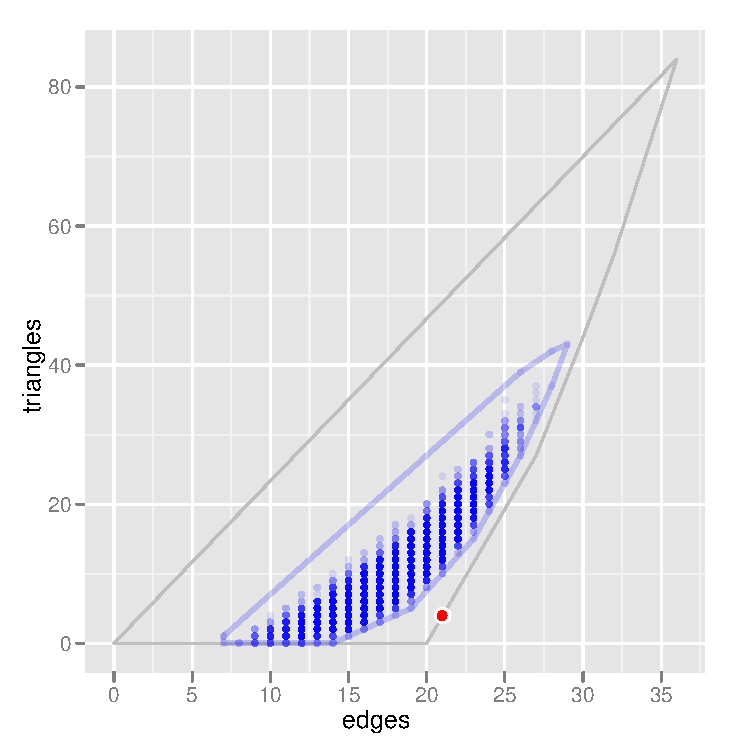
\includegraphics[height=2.4in,width=2.4in]{Figures/MCsample-problem}
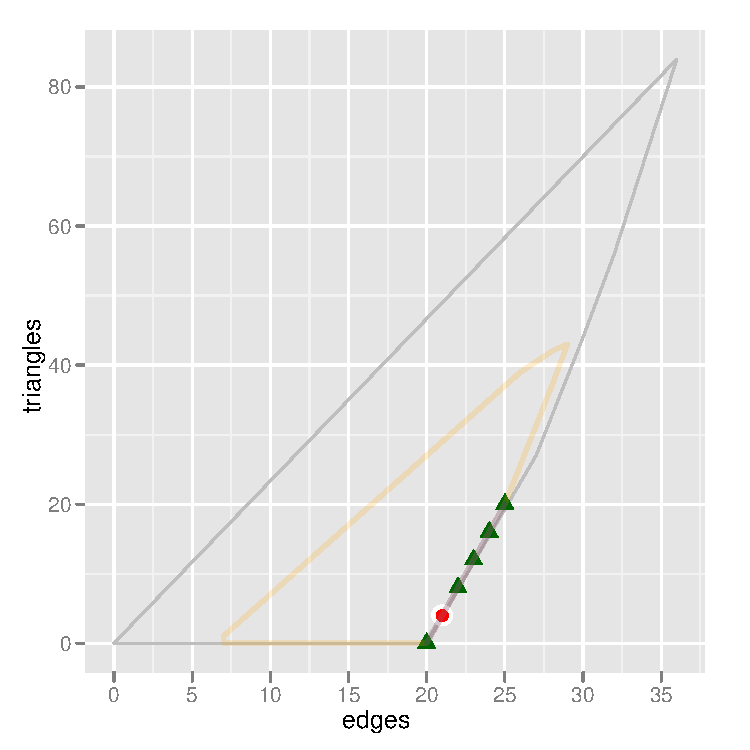
\includegraphics[height=4.5in,width=4.5in]{Figures/MCsample-fakeface}
\caption{An observed statistic at $(21,4)$, in the interior of the convex hull but 
close to the boundary.  It is quite feasible to generate 10,000 MC 
samples where all 10,000 points lie on a line segment that appear to be 
a one-dimensional face, marked by the triangles in the figure above.  
The lighter colored polytope is the convex hull of all previously 
sampled points used to derive this empirical face.}
\label{F:MC problem}
\end{figure}

Our algorithm treats the line segment as a boundary of the 
convex support on which the observed statistic lies in the relative interior, and 
concludes the MLE does not exist.  It does not stop there; it proceeds as in the first
example and seeks to find the MLE of the LCM,
\begin{align*}
	\etaLCM = (35.38, -9.39),
\end{align*}
after which it then calculates one-sided confidence intervals for $\eta$.

On first glance this is very troubling: our algorithm arrives at the wrong conclusion 
about the existence of the MLE, and $(35.38, -9.39)$ does not look close 
to the true MLE of $(28.86, -7.76)$.  However, we believe the algorithm is
actually performing better than it might initially appear.
A step back should be taken and the goal of the analysis revisited.  

What is the purpose in finding the MLE?  In particular, what does one do with these values once they are found?

If the end goal is to try to interpret meaning out of these numbers by their sign and  
magnitude, then we indeed have a problem---our numbers are just wrong.  
However, if the MLE is viewed as an 
index into a specific model that assigns the highest probability to the observed data,
then we claim that the model we have found---the LCM with parameter value $\etaLCM$---
is in fact remarkably similar to the original model indexed by the true MLE.  A 
reasonable metric for this comparison is a sum of the absolute difference in 
probabilities assigned to each point in the sample space,
\begin{align*}
	\sum_{y \in \YY} \abs{ P_{\etaMLE}(g(Y) =g(y) ) -  P_{\etaLCM}(g(Y) = g(y))  }.
\end{align*}
The probabilities assigned by each of these models to the six points on the 
empirically determined face is summarized in Table~\ref{T:LCMvsMLE}.

% latex table generated in R 2.11.1 by xtable 1.5-6 package
% Fri Sep 10 13:22:25 2010
\begin{table}[h!] 
\begin{center}
\caption{Probabilities assigned by LCM model with parameter value $\etaLCM$ and 
original model with parameter value $\etaMLE$ to the six points on the empirical face.  The observed statistic is $(21,4)$.  For the MLE model, the probability do 
not sum to 1 since it assigns positive probability to points other than these six.}

\begin{tabular}{rrrrr}
\\  \hline
 & Edges & Triangles & LCM & MLE \\ 
  \hline
1 & 20 & 0 & 0.3414 & 0.3425 \\ 
  2 & 22 & 8 & 0.2019 & 0.2009 \\ 
  3 & 21 & 4 & 0.3914 & 0.3911 \\ 
  4 & 23 & 12 & 0.0566 & 0.0561 \\ 
  5 & 24 & 16 & 0.0081 & 0.0080 \\ 
  6 & 25 & 20 & 0.0005 & 0.0005 \\ 
   \hline
   &  &  & 1.0000 & 0.9990 \\ 
\end{tabular}\label{T:LCMvsMLE}
\end{center}
\end{table}

Here, the sum of the absolute value of differences on these empirical points is only 
$0.0031$.  Including the additional 0.001 of probability on points that are outside 
the LCM support, this total still only comes to $0.0041$, a difference that would seem 
insignificant for most applications.  

Of course, there are practical issues: even if a researcher is interested in the 
MLE distribution, she may want the software to simply 
return MLE values to keep around for later analysis.  Here, we are suggesting that the 
analysis return LCM MLE values and an LCM model (perhaps in the form of the convex 
support).  The researcher may understandably be confused, especially if she knew in 
advance that the MLE was guaranteed to exist.  However, any distributional analysis 
would be almost identical, though perhaps not ``out of the box".

It may be of interest to note that $\etaLCM$ and $\etaMLE$ index nearly identical 
models in the LCM, with the difference due almost entirely to the lack of 
identifiability of the LCM.  A normal direction to the (incorrect) empirical face is 
$\delta = (4,-1)$, which is also a direction of constancy for the LCM. 
%(that is, $\delta \in \Gammalim$).  
Then by \eqref{E:Gammalim}, 
\begin{align*}
	\ell(\etaLCM)^{LCM} &= \ell( \etaLCM + \gamma )^{LCM}\\
				 &= 	\ell(\etaLCM + k \, (4,-1))^{LCM}.
\end{align*}
If we had perfect knowledge and chose $k = -1.63$,
\begin{align*}
	\etaLCM  -1.63 \, (4,-1)= (28.86, -7.76) 
\end{align*}
matching the MLE to the significant figures considered.  Thus in this case, $\etaLCM$ 
and $\etaMLE$ index nearly identical models of the LCM.

If we allowed the algorithm to finish the incorrect analysis and computed 
one-sided 95\% confidence intervals for $\eta$, we get 
\begin{align*}
%14.495152 -3.703202 
	[20.46, +\infty)\\
	(-\infty, -4.85].
\end{align*}
%20.462923 -4.850603 

%\begin{align*}
%	\hat{\theta}_{MLE} &= (28.85685, -7.75672)\\
%	\hat{\theta}_{LCM} &= (35.3831787, -9.387266),
%\end{align*}

%Well, remember that for LCM's we are looking to construct one-sided CIs.  But here, 
%what happens if we go off to infinity in this supposed direction of recession?  The 
%log-likelihood will eventually dip back down!  So, we can constructed two-sided CI's, 
%I think.  But, my calculations got me something that seems pointlessly wide: 
%\begin{align*}
% (3.503179,  -1.417266 )\\
% (71.22318,  -18.34727 ).
%\end{align*}

%%%%%%%%%%%%%%%%%%%%%%%%%%%%%%%%%%%%%%%%%%%%%%%%%%%%%
%\subsection{Three-dimensional sufficient statistic}
%In order to increase the complexity of the problem yet still have the ``truth" for 
%comparison, we also considered 7-node graph with network statistics edges, two-stars, 
%and triangles, a classic model in the literature first suggested by \citet{Frank:
%1986}.  Since then it has been criticized for its problematic behavior by \citet
%[really? check this]{GOF}, precisely related to the issue of non-existence MLEs (or 
%degeneracy???).
%
%The algorithm proceeds in exactly the same way, the difference now being that the 
%empirical face may have as many as two dimensions instead of one.  This makes for a 
%more interesting variety of constancy spaces for the LCM.  We only consider cases here 
%that add a notably different flavor than the two-dimensional case.
%
%\subsubsection{Observed value, $y_{obs}$, is on two-dimensional face}
%\subsubsection{Observed value, $y_{obs}$, is on one-dimensional face}
%\subsubsection{MLE does not exist; observed statistic on two-dimensional face but not 
%fully discovered}
%
%Set $y_{obs} = (14, 8, 43).$
%This point is on the boundary, which is a 2-dim face.
%
%The MC sample, however, does not cover the entire face.  This is a new scenario, but 
%it should not be a problem.  Those points on the actual face that are not included are 
%simply points of low probability.
%
%Only issue outstanding with this is how long it takes to find the LCM MLE.  Having a 
%surprisingly hard time with this.  Question: is it doing any worse than when we 
%started with a 2-dim sample space?

%\section{Example: \textit{e. coli}?}
\section{Example: Faux Magnolia High School} \label{S:FauxMagnolia}
\citet{advancesp*,statnet-tutorial} utilize a adolescent friendship network data set 
of 1,461 students in grade 7--12 derived from the National Longitudinal Study of 
Adolescent Health.  The data set, which \citeauthor{statnet-tutorial} refer to as Faux 
Magnolia High School, is a model-based simulation from the original data set, where 
the simulation is necessitated to maintain confidentiality.

\begin{figure}[!ht]
\centering
\includegraphics[width=5in]{Figures/fmh-grade}
\caption{Faux Magnolia High without isolates, colored by grade.  That data is available
in \texttt{ergm}.
}
\label{F:fmh}
\end{figure}

\subsection{MLE exists}
\citet{statnet-tutorial} run analyses and settle on a model with the following terms: 
Grade, Race, Sex, edges, and a geometrically weighted edgewise share partner (GWESP).\footnote{the model selection issue is one we do not address here.  See \citet{GOF}
 for methods of goodness-of-fit.}  
Grade, Race, and Sex are covariate factors specific to the 
actors and reflect whether or not the two actors in a dyad are of the same type.  
The incorporation of these into an ERGM was 
discussed in Section~\ref{S:Covariate}.  The GWESP statistic is not one we
have discussed previously but has been alluded to in Section~\ref{S:ERGM setup} as
one of the newly developed statistics designed to reduce degeneracy 
\citep{Handcock:2006, Hunter:2006, recentp*}.  This particular statistics can be 
thought of as a variant of triangles.

We run our algorithm through 40 search directions, starting from an initial value for 
$\eta$ of $(0, 0, 0, 0, 0)$.  As in the example with Sampson's monastery data, we rely
on the \texttt{simulate.formula} command provided in the \texttt{ergm} package to
generate our MCMC samples from the distributions indexed by $\eta$.  The results of our 
estimates are reported in Table~\ref{T:FauxMagnolia}.
%SEE PAGE 15
%\begin{verbatim}
%data("faux.magnolia.high")
%fmh <- faux.magnolia.high
%plot(fmh, displayisolates = FALSE, vertex.cex = 0.7)
%plot(fmh, displayisolates = FALSE, vertex.col = "Grade", vertex.cex = 0.7)
%R> summary(fmh ~ triangle)
%triangle 169
%Instinct tells us that 169 triangles is many more than would be expected by chance in a network of 1,461 actors and 974 edges. 
%
%> model3.take2 <- ergm(fmh ~ edges + triangle, MCMCsamplesize = 1e+5, 
%+	interval = 1000, verbose = TRUE, seed = 88)
%model3.take3 <- ergm(fmh ~ edges + triangle, maxit = 25, seed = 888,	
%control = control.ergm(steplength = 0.25), verbose = TRUE)
%
%R> model4.take3 <- ergm(fmh ~ edges + nodematch("Grade") +
%nodematch("Race") + nodematch("Sex") + gwesp(0.2, fixed = TRUE), 
%MCMCsamplesize = 1e+5, maxit = 15, verbose = TRUE, 
%control = control.ergm(steplength = 0.25), seed = 123)
%
%edges nodematch.Grade nodematch.Race	nodematch.Sex gwesp.fixed.0.2 
%-9.7915376	2.7557927	0.9184486	0.7664999	1.8150806
%\end{verbatim}

% latex table generated in R 2.12.1 by xtable 1.5-6 package
% Wed Mar  9 23:32:59 2011
\begin{table}[h]  
\begin{center} 
\caption{Coefficients estimates derived from using the default MCMC-MLE algorithm
in \texttt{ergm} through 5 iterations ($\etaMLE$ below) 
and our algorithm $\hat{\eta}_{\textrm{Steep}}$ through 40 iterations.}
\begin{tabular}{rrrrrr}
  \hline
 & edges & Grade & Race & Sex & GWESP \\ 
  \hline
$\etaMLE$ & -9.790 & 2.755 & 0.906 & 0.780 & 1.813 \\ 
$\hat{\eta}_{\textrm{Steep}}$ & -9.879 & 2.810 & 0.942 & 0.786 & 1.809 \\ 
   \hline
\end{tabular}\label{T:FauxMagnolia}
\end{center}
\end{table}

We compare our estimates to MLEs obtained by running the default MCMC-MLE algorithm 
in \texttt{ergm}, which starts from a MPLE of
\begin{align*}
	\hat{\eta}_{MPLE } = ( -9.8665, 2.8626, 0.9944, 0.8261, 1.6950 ).
\end{align*}
It is noteworthy that MCMC-MLE would have had exactly the difficulties 
described in Section~\ref{S:MCMC-MLE} if it were started at $(0, 0, 0, 0, 0)$ as well:
after 15 iterations, all the coefficient estimates would still effectively be zeros.
Thus its successful convergence here is due entirely to its use of 
a very good MPLE estimate, which cannot always be relied upon.

Our algorithm is very time consuming.  Whereas running MCMC-MLE through 15 iterations with MCMC sample sizes of 100,000 at intervals of 100 steps as done 
by \citet{statnet-tutorial} takes only a few minutes, 
we used over 100 iterations over 40 search directions, 
each iteration using MCMC sample sizes of 
10,000 spaced 5,000 iterations apart, taking over an hour.  We actually stopped the 
algorithm at 40 search direction; we did not attain our desired cutoff value for 
$\lVert \nabla \ell(\eta) \rVert < 0.01$ and were only able to 
attain values as small as $9.6$.
 
A few remarks:
\begin{itemize}
\item The goal here is to show that our algorithm can in fact find the MLE if needed, 
starting from any initial value for a more realistic model and a large data set.  
Although it is not computationally expedient, 
we obtain a reasonable estimate after 40 search directions.  That the network
is large is a concern for the MCMC sampler and not our algorithm, which is only
dealing with a five dimensional parameter.

\item Our recommended use of this algorithm is in combination with other algorithms,
as discussed in Section~\ref{S:Combine}.  Thus, although it is satisfying to see a reasonable estimate of the MLE, what is more useful is the value of $\eta$ 
at say $2d$ iterations, where $d$ is the dimension of $\eta$.  
Here we see that at 10 iterations,
\begin{align*}
	\eta_{10} =( -8.330,  2.462,  0.565,  0.430,  0.879) 
\end{align*}
which makes for a good starting point for MCMC-MLE to converge in 1 iteration.
Using conjugate gradient directions here does even better, with
\begin{align*}
	\eta_{10} =( -9.963,  2.965,  0.927,  0.742,  1.784).
\end{align*}
\item MCMC sampler.  We have developed our algorithm assuming that it would have access
to a reasonably efficient MCMC sampler.  In this example, we found that the MCMC
sampler performs much better with a larger interval between samples.  This is unsurprising given the very large number of nodes (1461 actors) 
and the challenging issues of generating less dependent discrete samples.  
%In fact,
%our brief experience with this sampler, it would seem that the default 100 interval 
%used may not have been sufficient.  

\item MCMC sample sizes.  A more pragmatic way to implement our algorithm would have
been to increase the MCMC sample sizes as the algorithm progressed.  That is, when
we are very far away, crude estimates of the gradient and step size should be sufficient
to get $\eta$ ``closer" and satisfy the curvature condition \eqref{E:Wolfe-ll}.
As noted in Section~\ref{S:MCMC approx}, when $\lVert \nabla \ell(\eta) \rVert$ gets
smaller, the curvature condition is more difficult to satisfy and sharper estimates---resulting from larger MCMC sizes---are necessary.
\end{itemize}


%\subsection{Degenerate}
%\citet{statnet-tutorial} also considered the edges-triangles model, and concluded
%that it is degenerate because the fitted model with coefficients $(-7.31, 4.504)$
% generates samples that look nothing like the observed data.  
% We apply our algorithm to this setting to see if we can detect a non-existent MLE.
 
